\documentclass[11pt, oneside]{article}   	% use "amsart" instead of "article" for AMSLaTeX format
\usepackage{geometry}                		% See geometry.pdf to learn the layout options. There are lots.
\geometry{letterpaper}                   		% ... or a4paper or a5paper or ... 
%\geometry{landscape}                		% Activate for for rotated page geometry
%\usepackage[parfill]{parskip}    		% Activate to begin paragraphs with an empty line rather than an indent
\usepackage{graphicx}				% Use pdf, png, jpg, or eps§ with pdflatex; use eps in DVI mode
								% TeX will automatically convert eps --> pdf in pdflatex		
\usepackage{amssymb}
\usepackage{amsmath}
\usepackage{parskip}
\usepackage{color}
\usepackage{hyperref}

\title{Complex functions:  square and higher roots}
%\author{The Author}
%\section{}
%\subsection*{}
\date{}							% Activate to display a given date or no date

\graphicspath{{/Users/telliott_admin/Dropbox/Tex/png/}}
% \begin{center} 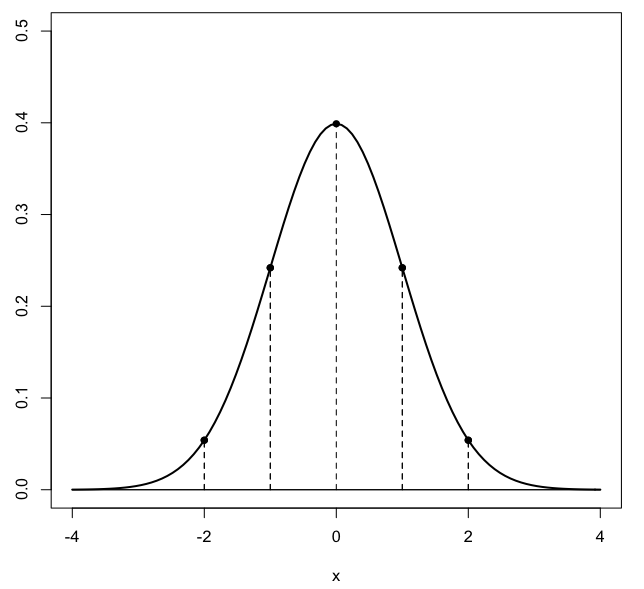
\includegraphics [scale=0.4] {gauss3.png} \end{center}
\begin{document}
\maketitle
\Large
Consider the square root function $\sqrt{z}$.  For the modulus part, we see that $\sqrt{r} \cdot \sqrt{r}$ is obviously equal to $r$, and what we need to determine the argument is to find an angle that is one-half of the original one, which leads us to
\[ \sqrt{z} = \sqrt{re^{i\theta}} = \sqrt{r} \ e^{i (\theta/2)} \]

However, recall from trigonometry (and what we said above) that $\theta + 2k \pi$ is the same angle as $\theta$, for integer $k$ ($k \in \mathbb{Z}$).

The same thing is true here.  It is allowed that $\theta ' = (2k \pi + \theta)$ for $k \in \{ 0, \pm 1, \pm 2 \dots \}$, since the result maps to the same point in the plane.

This means that a second solution to the square root problem is
\[ \sqrt{re^{i\theta}} = \sqrt{r} \ e^{i (\pi + \theta/2)} \]
because, again, $\sqrt{r} \cdot \sqrt{r} = r$ and
\[ \ e^{i (\pi + \theta/2)} \cdot \ e^{i (\pi + \theta/2)} = e^{i (2\pi + \theta)} = e^{i\theta} \]

For the square root, there is only one additional distinct solution, since one-half of $4 \pi + \theta = 2 \pi + \theta/2$ which is no different than $\theta/2$, but the cube root has 3 solutions and in general the $n^{th}$ root has $n$ solutions.

Consider points on the unit circle with $r=1$ (so $\sqrt{r} = r$) and suppose
\[ \theta = \pi/2 \]
so
\[ z = e^{i \pi/2} \]
Points with $\theta = \pi/2$ lie directly above the origin on the imaginary axis (there is no real component).  This point is one unit from the origin so it is the point $(0 + i \cdot 1) = i$.  Thus
\[ e^{i \pi/2} = i \]
Note that
\[ (e^{i \pi/2})^2 = e^{i (\pi/2 + \pi/2)}\]
\[ = e^{i\pi} = -1 = i^2 \]
We can justify this last step by geometry ($\theta = \pi$), or by using Euler's equation
\[ e^{i\theta} = cos \theta + i \sin \theta \]
\[ e^{i\pi} =  cos \pi + i \sin \pi = - 1 + i \cdot 0 = -1 \]

$\sqrt{e^{i \pi/2}} = \sqrt{i}$ has two possible values.  One is
\[ \sqrt{e^{i\pi/2}}  = (e^{i\pi/2})^{1/2} = e^{i\pi/4} \]
Let's just check.  The point is at a distance $1$ from the origin and angle $\theta = \pi/4$.  We go equal distances along the real and imaginary axes:
\[ x = \cos \theta = \frac{1}{\sqrt{2}} \]
\[ y = \sin \theta = \frac{1}{\sqrt{2}} \]
So we have that the square is:
\[ (\frac{1}{\sqrt{2}} + i \frac{1}{\sqrt{2}} )^2 = \frac{1}{2} - \frac{1}{2} + 2 i \frac{1}{2} \]
\[ = 0 + i = i \]
the second solution is
\[ \sqrt{e^{i\pi/2}}  = e^{i \cdot 5/4 \pi} \]
which can be plotted as
\[ x = \cos \theta = -\frac{1}{\sqrt{2}} \]
\[ y = \sin \theta = -\frac{1}{\sqrt{2}} \]
The square is the same except the first term is $(- 1/\sqrt{2})^2$, so the result is unchanged.  It's a bit counter-intuitive that squaring a number may possibly reduce the phase angle, but you can think of it as modular arithmetic (mod $2 \pi$).

In general, if we're working with the complex number
\[ re^{i\theta} \]
and we want the nth root, the modulus is just
\[ \rho = r^{1/n} \]
And the question always is, what's the angle?
\[ \phi = \frac{\theta + 2k\pi}{n}, \ \ \ k = 0, 1, 2 \dots n-1 \]

Let's say we want the cube roots of $1$.  Obviously, all the roots will have length $1$.  What about the angles?  The starting angle $\theta = 0$, so $\phi = 2k\pi/3$ and 
\[ \phi_ 1= \frac{2 \pi}{3} \]
\[ \phi_2 = \frac{4 \pi}{3} \]
\[ \phi_3 = \frac{6 \pi}{3} = 0 \]
Notice that the first and second roots are complex conjugates because
\[ \phi_1 + \phi_2 = \frac{6\pi}{3} = 2 \pi = 0 \]

Suppose our number is $z = -8i$ and we want the cube roots.  Writing the number in polar coordinates:
\[ z = 8e^{3\pi/2} \]
All of the roots have the same modulus, $2$, since $2^3 = 8$.  The are three roots which differ in their arguments.  Since $\theta = 3 \pi / 2$, these are:
\[ \phi_1 = \frac{\theta}{3} = \frac{\pi}{2} \]
\[ \phi_2 = \frac{\theta + 2\pi}{3} = \frac{\pi}{2} + \frac{2\pi}{3} = \frac{5\pi}{6} \]
\[ \phi_3 = \frac{\theta + 4\pi}{3} = \frac{\pi}{2} + \frac{4\pi}{3} = \frac{7\pi}{6} \]
Notice that the second and third roots are complex conjugates.

When the argument for $z$ is $\theta_0$, a general formula for the angle of the $nth$ root of $z$ is:
\[ \theta = \frac{\theta_0}{n} + \frac{2k\pi}{n} \ \ \ k = 0, \pm 1, \pm 2 \dots \]

We derive this as follows:
\[ z = r e^{i \theta} \]
\[ z^{1/n} = (r e^{i (\theta + 2k \pi)} )^{1/n} \]
Writing only the argument part
\[ (e^{i (\theta + 2k \pi)} )^{1/n} = e^{i (\theta/n + 2k \pi/n)}  \]

\subsection*{Nahin's puzzle}
In one of his books Nahin starts by posing this question:  suppose we are given that 
\[ x + \frac{1}{x} = 1 \]
\emph{Without computing} $x$, find the value of
\[ x^7 + \frac{1}{x^7} \]
Nahin says that if you are the type to just start right in trying to figure this out, then you will like his book.

From its placement in this section, you might just guess the answer.  First of all, no real $x$ solves the equation
\[ x + \frac{1}{x} = 1 \]
as you will see if you use the quadratic formula.  So let's change nomenclature and call it $z$.  (Of course, we were not supposed to \emph{compute} $z$).

We may guess that $z$ is a complex number with length $1$ so that the lengths don't change with powers or roots.  

Then, all that happens is that $\theta$ changes in such a way that 
\[ 7 \theta = \theta = \frac{\theta}{7}  \]

To actually compute $z$, multiply by $z$, rearrange, and solve:
\[ z^2 + 1 = z \]
\[ z^2 - z + 1 = 0 \]
From the quadratic equation:
\[ z = \frac{1 \pm \sqrt{1 - 4}}{2} = \frac{1}{2} \pm i \frac{\sqrt{3}}{2}  \]
The square of the length is
\[ r^2 = zz* \]
\[ = (\frac{1}{2} + i \frac{\sqrt{3}}{2}) (\frac{1}{2} - i \frac{\sqrt{3}}{2})  \]
\[ = \frac{1}{4} + \frac{3}{4} = 1 \]
The angle we seek has tangent equal to $1/\sqrt{3}$.  You may recognize the sine and cosine of $\pi/3$ as the real and imaginary components of $z$.

So if 
\[ z = e^{i \pi/3} = (\frac{1}{2} + i \frac{\sqrt{3}}{2}) \]
\[ \frac{1}{z} = e^{-i \pi/3} = (\frac{1}{2} - i \frac{\sqrt{3}}{2}) \]
then when doing the addition the imaginary parts of $z$ cancel and we have that 
\[ z + \frac{1}{z} = \frac{1}{2} + \frac{1}{2} = 1 \]

The other special attribute of this value for $z$ is that the length is $1$ so all powers of $r$ are $1$.  As for the angle, $\pi/3$ is special in that $7 \times \pi/3 = 2 \pi + \pi/3 = \pi/3$.  Now it's not strictly true that \emph{the} 7th root of $\theta$ is equal to $\theta$ (since there are 7 distinct roots).  But I hope you can see that there is at least one such root.

\end{document} 